\documentclass[12pt,a4paper]{article}
\usepackage[utf8]{inputenc}
\usepackage{graphicx}
\usepackage{geometry}
\usepackage{enumitem}
\usepackage{titlesec}
\usepackage{hyperref}

\geometry{margin=2.5cm}

\title{Course Analysis}
\date{}

\begin{document}

\maketitle

\section*{1. Overall Course Popularity}
According to Figure~\ref{fig:most-popular-courses}, Barista courses are by far the most popular, attracting 104 students, followed by Pizza (69 students) and Burger (51 students). Courses such as Traditional, Kabab, and Fried Chicken attract fewer students, suggesting limited demand or more specialised interest.

\begin{figure}[h!]
    \centering
    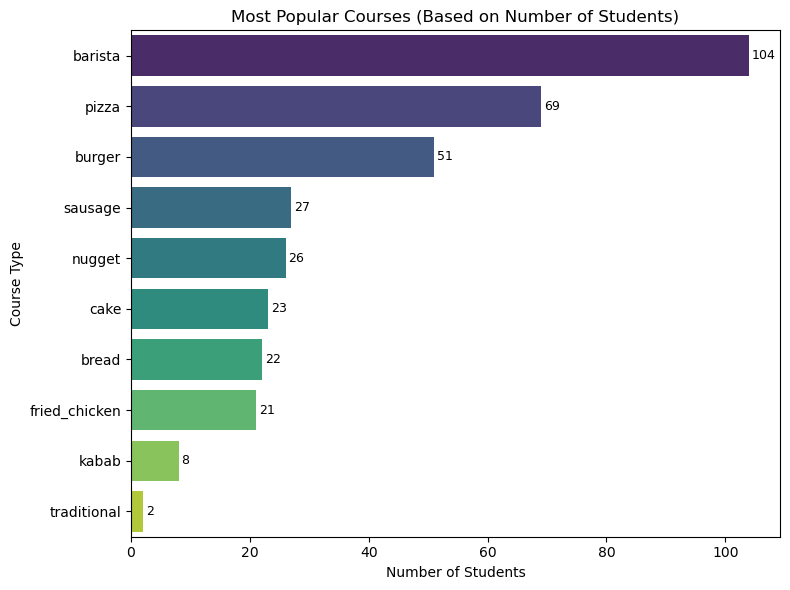
\includegraphics[width=0.8\textwidth]{Most Popular Courses (Based on Number of Students).png}
    \caption{Most Popular Courses (Based on Number of Students)}
    \label{fig:most-popular-courses}
\end{figure}

\section*{2. Seasonal Distribution of Students per Course}
As illustrated in Figure~\ref{fig:seasonal-courses}, Barista maintains consistent popularity across all seasons, peaking in summer.  
Pizza also performs strongly throughout the year with the highest count in summer.  
Some courses, such as Bread and Kabab, show higher enrolment mainly in autumn, pointing to seasonal preferences or scheduling choices.  
Courses like Traditional appear only in spring, which suggests they are one-off or experimental offerings.

\begin{figure}[h!]
    \centering
    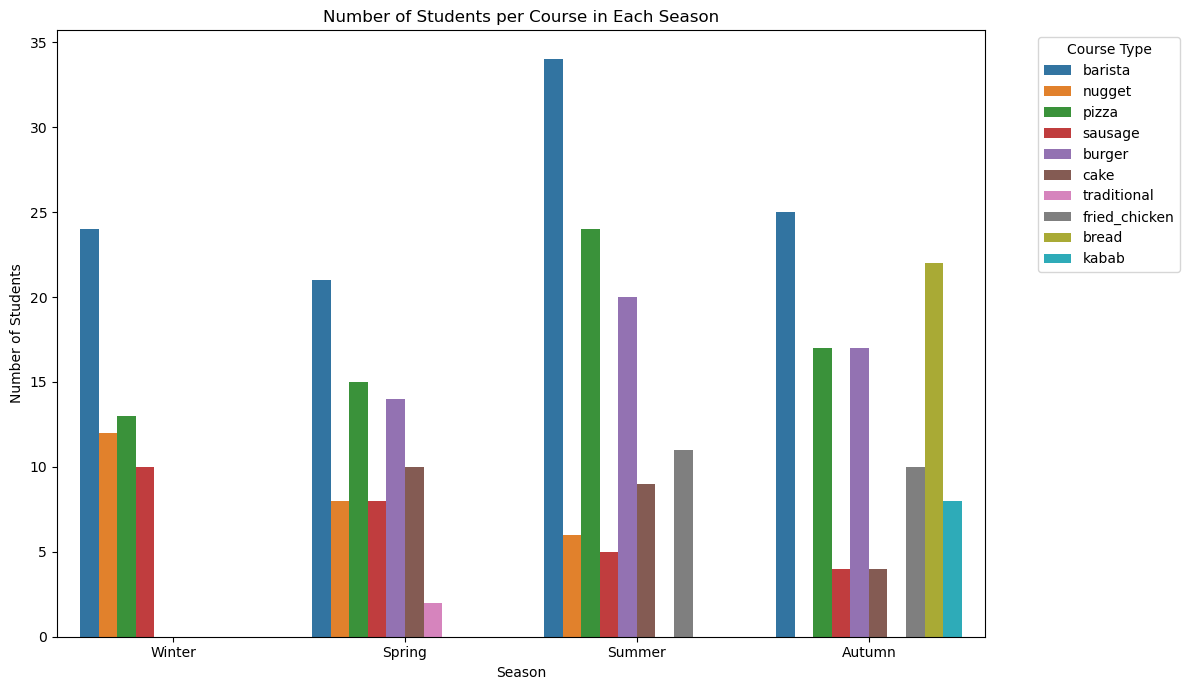
\includegraphics[width=1\textwidth]{Number of Students per Course in Each Season.png}
    \caption{Number of Students per Course in Each Season}
    \label{fig:seasonal-courses}
\end{figure}

\section*{3. Monthly Dynamics by Course Type}
The heatmap in Figure~\ref{fig:heatmap-course-month} provides a detailed view of course engagement across time:  
Barista and Pizza have consistently high participation every month, especially in July and November.  
Burger courses peaked in May, July, and November.  
Several lower-enrolment courses have patchy presence (e.g., Traditional only appears once).  
The heatmap highlights summer and autumn as peak periods, when a broader range of courses is in demand.

\begin{figure}[h!]
    \centering
    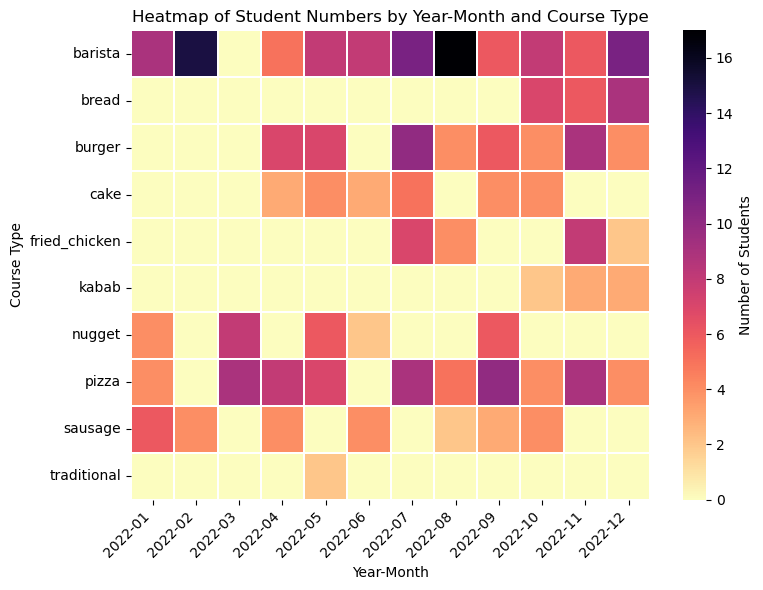
\includegraphics[width=1\textwidth]{Heatmap of Student Numbers by Year-Month and Course Type.png}
    \caption{Heatmap of Student Numbers by Year-Month and Course Type}
    \label{fig:heatmap-course-month}
\end{figure}

\section*{Summary}
Barista and Pizza dominate in terms of student interest and consistency.  
Seasonality influences the demand for some courses, notably in summer and autumn.  
A few courses have sporadic or limited availability, possibly due to resource constraints or experimental offerings.

\end{document}